\chapter{\chapternamedatabase}\label{database}


\section{S-PLUS}
O Southern Photometric Local Universe Survey (S-PLUS), um levantamento do céu do hemisfério Sul, localizado no Cerro Tololo Inter-American Observatory, Chile (CTIO), tem como objetivo observar uma área de 9300 graus quadrados com o telescópio robótico de 80cm (T80-South). Ele disponibiliza 12 filtros fotométricos (Figura \ref{splus_filters}), sendo 5 de banda larga ($u$, $g$, $r$, $z$) e 7 de banda estreita (J0378, J0395,
87 J0410, J0430, J0515, J0660 e J0861).

\vspace{\baselineskip}

Os dados utilizados neste trabalho foram obtidos a partir do quarto lançamento de dados do S-PLUS (DR4) \cite{herpich2024fourthsplusdatarelease}. O DR4 cobre uma área de 3022.7 graus quadrados, composto por 1629 campos, canda um deles com um campo de visão de aproximadamente 2 graus quadrados. A Figura \ref{footprint_iDR4} mostra a área coberta pelo S-PLUS DR4.

\begin{figure}[!ht]
    \begin{center}
    % \setcaptionmargin{1cm}
    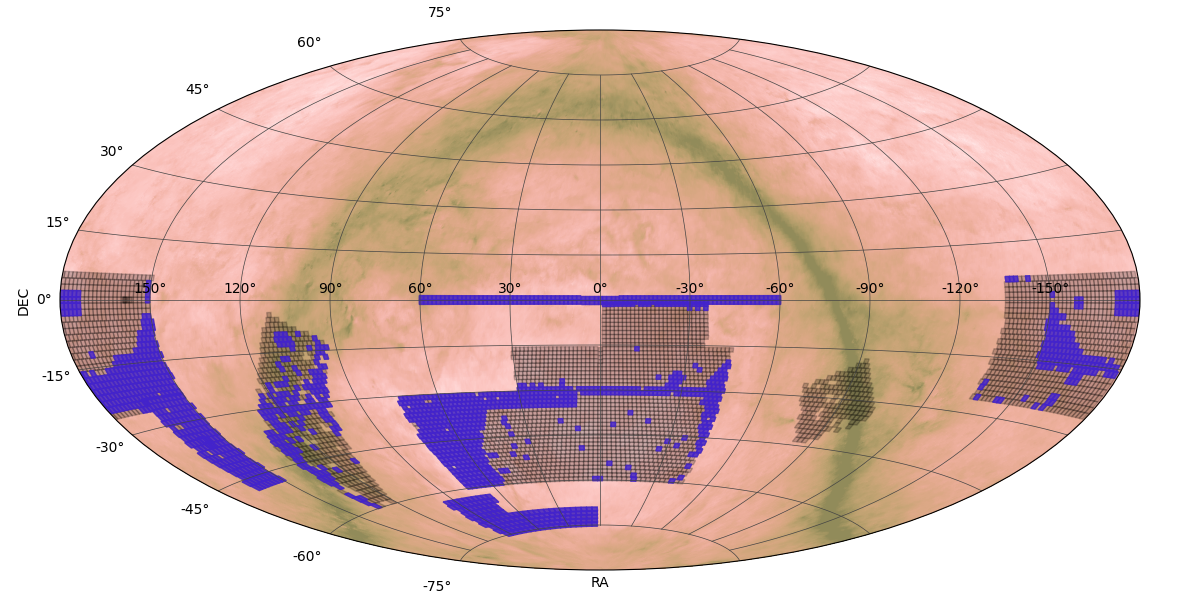
\includegraphics[width=1.0 \columnwidth,angle=0]{footprint_iDR4.png}
    \caption[]{Área coberta pelo S-PLUS DR4. Campos em azul foram observados, enquanto campos em cinza não foram observados \cite{splus_DR4_footprint}.}
    \label{footprint_iDR4}
    \end{center}
\end{figure}

Além dos 12 filtros fotométricos mencionados, temos opções de aberturas fotométricas para cada uma dessas bandas. Entre as aberturas disponíveis, destacam-se:

\begin{itemize}
    \item \textbf{ISO}: Captura o fluxo dentro de uma isofota, definida por um limite de brilho constante.
    \item \textbf{PETRO}: Mede o fluxo utilizando a abertura de Petrosian, que captura uma fração constante da luz total da galáxia, minimizando a perda de luz nas regiões externas.
    \item \textbf{AUTO}: Abertura adaptativa que utiliza um algoritmo automático para ajustar a abertura ao tamanho e forma do objeto.
    \item \textbf{APER\_3}: Abertura fixa de 3 pixels de raio, adequada para medir o fluxo em regiões centrais.
    \item \textbf{APER\_6}: Abertura fixa de 6 pixels de raio, usada para capturar uma área maior do objeto, balanceando entre evitar contaminação de fontes próximas e capturar mais do fluxo total.
\end{itemize}

Para este trabalho, escolhemos utilizar as magnitudes baseadas na abertura PETRO (ex.: u\_PETRO, J0378\_PETRO etc.). A escolha foi motivada pela necessidade de uma medida consistente e confiável da luz total dos objetos.

\begin{figure}[!ht]
    \begin{center}
    % \setcaptionmargin{1cm}
    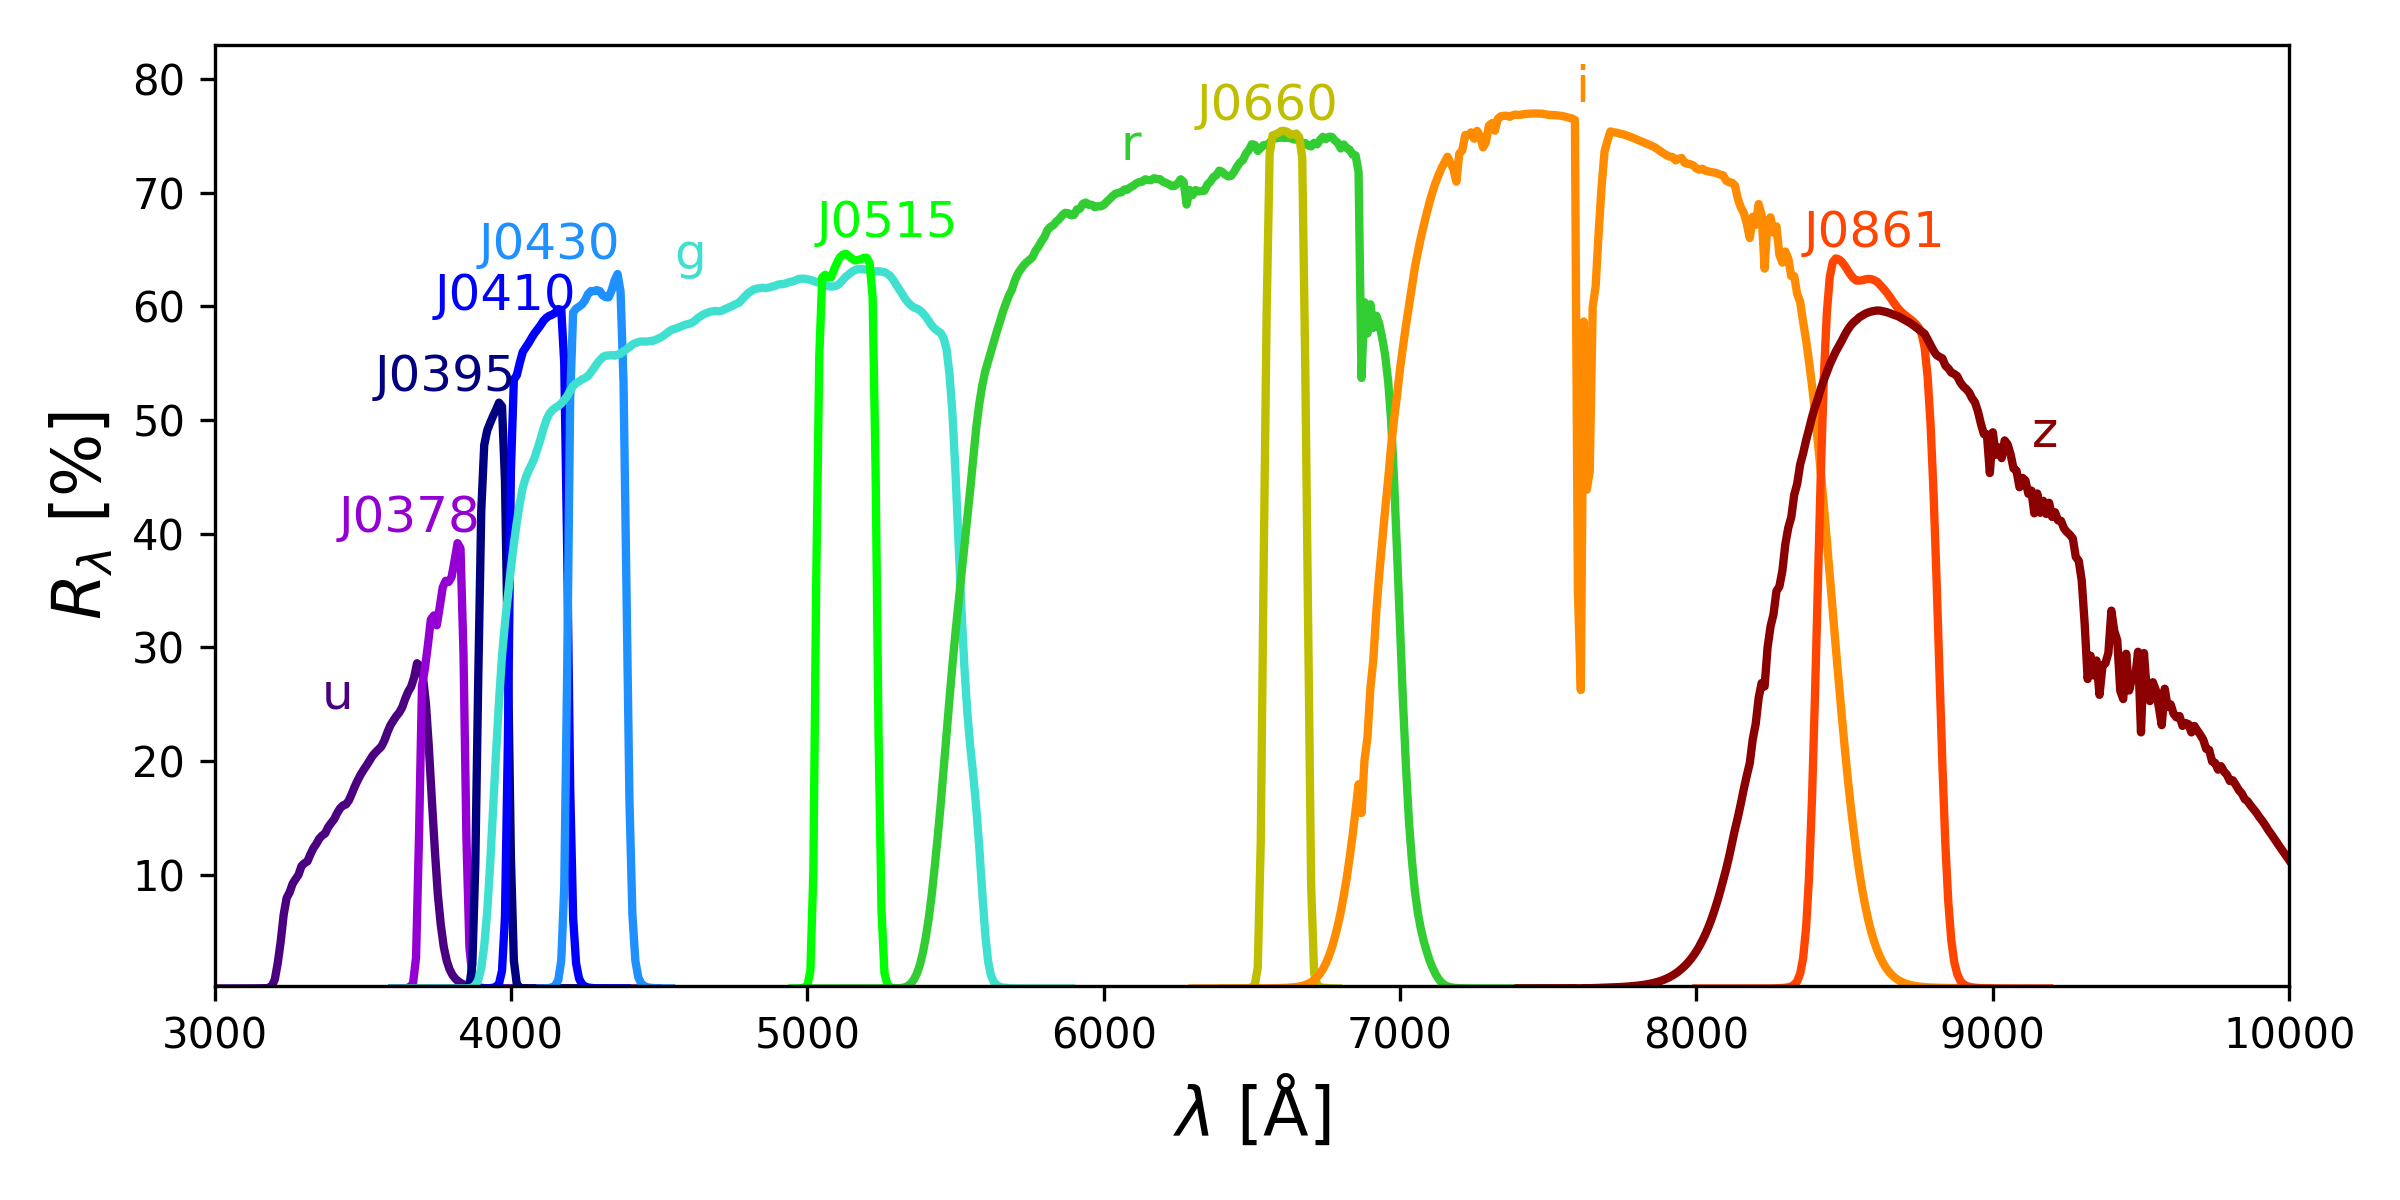
\includegraphics[width=1.0 \columnwidth,angle=0]{splus_filters.png}
    \caption[]{Comprimentos de onda efetivo dos 12 filtros fotométricos do S-PLUS (\cite{splus_DR4_footprint}).}
    \label{splus_filters}
    \end{center}
\end{figure}

\subsection{Fornax Data}
\label{sec:Fornax_data}
Os dados do aglomerado de Fornax foram obtidos a partir da mesma fonte que os dados do S-PLUS, o DR4. Porém, a partir da colaboração de \cite{castelli2024splusfornaxprojectsfp},utilizamos os dados de \cite{haack2024splusfornaxprojectsfp}, onde foram utilizadas novas execuções específicas do SExtractor, identificando o  conjunto mais adequado de parâmetros para recuperar o máximo possível de galáxias Fornax com fotometria confiável e evitando duplicações.

\vspace{\baselineskip}

Os parâmetros da RUN 1 foram projetados para identificar galáxias fracas e objetos compactos próximos a galáxias mais brilhantes. Por outro lado, os parâmetros da RUN 2 são voltados para uma boa caracterização de galáxias brilhantes e extensas. Assim, para detectar objetos compactos como anãs ultra-compactas (UCDs) ou aglomerados globulares (GCs) perto das galáxias de Fornax, os parâmetros da RUN 1 são mais adequados. Já para caracterizar melhor os objetos mais brilhantes e extensos em Fornax, os parâmetros da RUN 2 são mais eficazes. No nosso caso, usamos os dados da RUN 1.

\vspace{\baselineskip}

\subsection{Correção da extinção}
\label{sec:Coeficientes_ext}
As magnitudes fornecidas pelo S-PLUS DR4 não estão corrigidas para a extinção interestelar. A poeira galáctica pode afetar bastante as medições fotométricas, principalmente em áreas do céu com alta densidade de poeira. Para garantir que os dados fotométricos que usamos sejam precisos, é necessário aplicar uma correção de extinção.

\vspace{\baselineskip}

Através do pacote Python 'dustmaps' (\cite{dustmapsGreen2018}), utilizamos o map de poeira CSFD (\cite{chiang2023correctedsfdaccurategalactic}).  O mapa CSFD é uma versão melhorada do mapa de Schlegel-Finkbeiner-Davis (SFD) (\cite{Schlegel_1998}; \cite{Schlafly_2011}), que é comumente utilizado para estimar a extinção em diferentes direções do céu. A correção fornecida pelo CSFD ajuda a reduzir os efeitos da estrutura em larga escala e da contaminação do fundo infravermelho cósmico (CIB). Com esses efeitos removidos, o mapa CSFD da um valor mais preciso e confiável da extinção interestelar.

\vspace{\baselineskip}

\subsubsection*{Cálculo dos Coeficientes de Extinção}
Para converter as estimativas de extinção fornecidas pelo mapa de poeira em correções aplicáveis às magnitudes fotométricas, utilizamos a lei de extinção de \cite{cardelli1989dust}. Para cada uma das 12 magnitudes, calculamos os coeficientes de extinção com base nos comprimentos de onda efetivos das respectivas bandas.

\sloppy
O cálculo dos coeficientes de extinção foi feito utilizando o pacote Python \texttt{extinction} \cite{barbary2017extinction}, que implementa a lei de \cite{cardelli1989dust} e permite a aplicação direta das correções de extinção às magnitudes observadas.

\section{GEMINI}
O Observatório Gemini é uma instalação astronômica internacional composta por dois telescópios gêmeos: um localizado no hemisfério norte, no Havaí, e outro no hemisfério sul, no Chile. O Gemini South, situado no Chile, é equipado com um espelho primário de 8,1 metros de diâmetro.

Para a busca por novas galáxias ultracompactas no aglomerado de Fornax, a partir das candidatas identificadas pela metodologia adotada neste trabalho, é necessário realizar confirmações espectroscópicas. Essas confirmações são importantes para observar se as candidatas são de fato galáxias, e se elas estão no redshift do aglomerado de Fornax. Para isso, utilizamos dados espectroscópicos obtidos do GMOS-S, instalado no telescópio Gemini South.

\vspace{\baselineskip}

Como parte deste projeto, algumas candidatas preliminares já haviam sido selecionadas em um trabalho de iniciação científica anterior. Nesse contexto, analisamos os dados espectroscópicos dessas candidatas prévias, além de solicitar e analisar novos dados espectroscópicos obtidos para as novas candidatas identificadas neste estudo.

\vspace{\baselineskip}

Os dados espectroscópicos foram obtidos através do repositório online do Gemini Observatory\footnote{Gemini Observatory, \textit{Gemini Observatory Archive}, disponível em \url{https://archive.gemini.edu}}. Para a análise das candidatas a galáxias ultracompactas (UCDs) no aglomerado de Fornax, foram utilizadas as seguintes configurações:

\begin{itemize}
    \item \textbf{Telescópio}: GMOS-S no Gemini South.
    \item \textbf{Modo de Observação}: Modo de fenda longa.
    \item \textbf{Gratinete}: B600-G5303 com comprimento de onda central $\lambda_c = 550 \, \text{nm}$ e fenda de 1,500 $\mu\text{m}$.
    \item \textbf{Intervalo Espectral}: [4000\,\text{Å} - 7000\,\text{Å}]
    \item \textbf{Resolução}: $R \approx 570$.
    \item \textbf{Tempo de Exposição}: 1200 segundos por alvo
    \item \textbf{S/N Desejada}: Mínimo de 5 no continuum (S/N $\sim$ 3 por pixel espectral) e S/N $\sim$ 20 nas linhas de emissão.
\end{itemize}
